
\chapter{Implementation}
\epigraph{The trouble with opportunity is that it always comes disguised as hard work.}%
{\textsc{---herbert v.\ prochnow}}


%\begin{itemize}
%\item implementing parallel algorithms (20\%, 1 week)
%    \begin{itemize}
%        \item fold
%        \item scan
%        \item permute (atomic operations)
%        \item segmented/rank polymorphic operations
%    \end{itemize}
%
%\item skeleton-based code generation (2 weeks)
%    \begin{itemize}
%        \item device capabilities (free array variables, \code{umul24},
%            \code{shfl}, atomic operations, shared memory)
%        \item rank polymorphic operations
%    \end{itemize}
%
%\item runtime system (3 weeks)
%    \begin{itemize}
%        \item launching kernels (occupancy calculator)
%        \item caching compiled kernels (live \& persistent caches)
%        \item memory management (escaping the EDSL evaluator; weak pointers vs.
%            reference counting)
%        \item executing kernels (annotated AST)
%    \end{itemize}
%
%\end{itemize}

% \begin{itemize}
%\item Accelerate frontend
%    \begin{itemize}
%        \item reification
%            \begin{itemize}
%                \item smart constructors for type classes
%                \item explicit dictionaries (polymorphism)
%                \item environments
%                \item HOAS vs. de Bruijn
%                \item representation types
%            \end{itemize}
%        \item surface \& internal (core) languages
%            \begin{itemize}
%                \item representing different constructs in surface/core
%                \item surface nested $\rightarrow$ core flat ?? (fuuuuture)
%            \end{itemize}
%        \item sharing observation ( --> sec 5? not my work )
%    \end{itemize}
%
%\item Accelerate CUDA backend
%    \begin{itemize}
%        \item code generation
%            \begin{itemize}
%                \item architecture sensitive JIT cross-compiler
%                \item future work: types, Haskell compile time
%            \end{itemize}
%        \item external compilation
%            \begin{itemize}
%                \item annotating AST nodes
%            \end{itemize}
%        \item memory management
%            \begin{itemize}
%                \item weak pointers \& weak hash tables
%                \item advantages to alternatives
%            \end{itemize}
%        \item execution
%            \begin{itemize}
%                \item occupancy analysis
%                \item multi-pass kernels
%            \end{itemize}
%        \item performance
%            \begin{itemize}
%                \item amortizing overheads (how to quantise this?)
%                \item of generated code
%                \item runtime overheads
%                \item w.r.t. CUDA memory subsystem (theoretical performance)
%                \item examples! spot the infelicities! (dot product)
%            \end{itemize}
%    \end{itemize}
%\end{itemize}

%Compilation has five phases:
%\begin{itemize}
%    \item Lexing
%    \item Parsing
%    \item Semantic analysis
%    \item Optimisation
%    \item Code Generation
%\end{itemize}

The previous chapter described the design of the Accelerate language, an
embedded DSL of operations over arrays, rich enough to express some interesting
real-world problems. This chapter details the architecture of the embedding as
well as the implementation of a backend for parallel execution on CUDA hardware.

\section{Implementing Parallel Algorithms}


\subsection{Reduction}
\label{sec:parallel_reduction}

Reductions are a common and important data-parallel primitive.
Figure~\ref{fig:tree_reduction} illustrates the basic strategy of a tree
reduction: within each thread block a tree-based approach is used to reduce
elements to a single value, and multiple thread blocks each process a portion of
the array in parallel. There is no global synchronisation primitive in CUDA,
because (a) it would be expensive to build in hardware for large numbers of
multiprocessors, and (b) would be difficult for programmers to use without
introducing sources of deadlock. Instead, kernel launches serve as a global
synchronisation point, so thread blocks instead communicate their partial
results by committing them to memory, and the kernel is launched recursively
until the final reduction is computed.

\begin{figure}[htbp]
    \begin{center}
        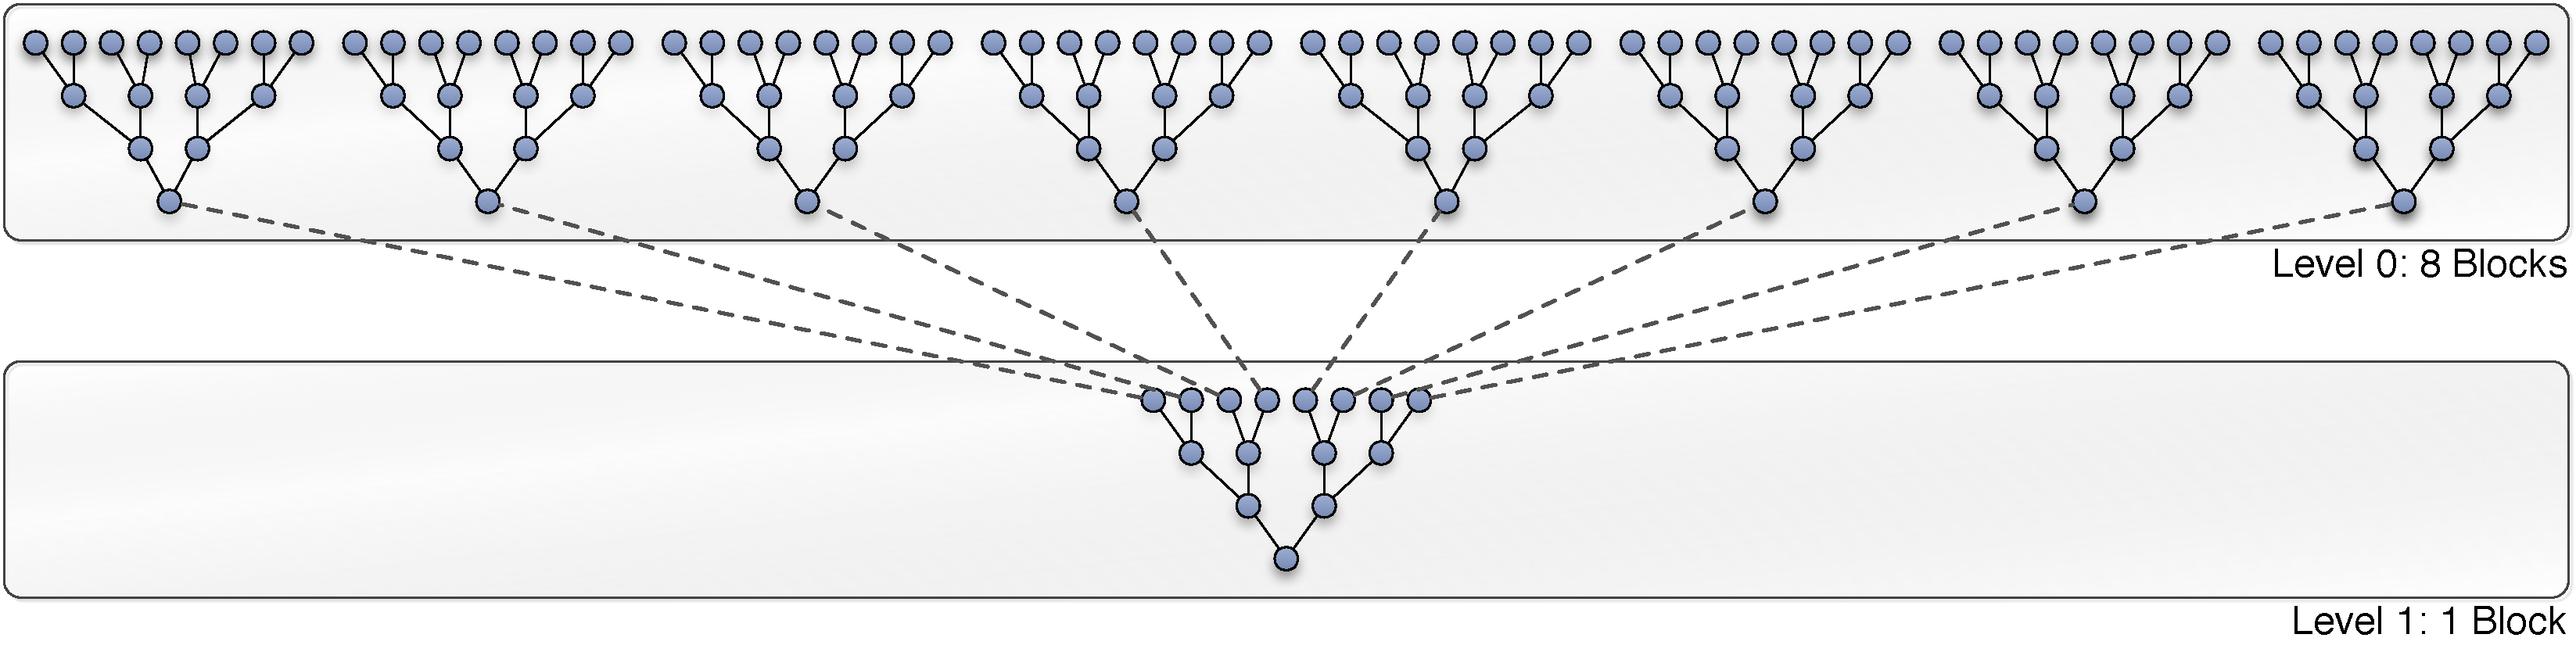
\includegraphics[width=\textwidth]{images/sec-4/tree-reduction}
    \end{center}
    \caption[A parallel tree reduction]{Illustration of a tree reduction,
        performed in two steps. In the first step 8 thread blocks in parallel
        reduce 8 elements to a single value. The thread blocks synchronise by
        writing their result to memory, and the kernel is called recursively
        until the final result is computed.}
    \label{fig:tree_reduction}
\end{figure}

For a fused dot product kernel, only the first line of reductions at level zero
perform the element wise multiplication. All subsequent reductions in that
kernel, as well as the recursive steps at level one and beyond, are pure
reductions. Thus, the fused operation requires compilation of two separate
kernels. % We focus on the level zero kernel, which is more interesting.

\subsubsection{Parallel Reduction Complexity}
\label{sec:parallel_reduction_complexity}

If each thread combines two elements at a time, then a vector of length $N$ will
\marginnote{tk: for power-of-2 n, add upper/lower bounds symbols}
be reduced in $\mathcal{O}\left( \log N \right)$ parallel steps. Each step $S$
does $\sfrac{N}{S^2}$ independent operations, so the \emph{step
complexity}\index{complexity!step} of the algorithm is:
\[
\mathcal{O}\left( \log N \right)
\]
For $N=2^{D}$, the algorithm thus performs $\sum_{S=1}^{D}2^{D-S} = N - 1$
operations. This means that the \emph{work complexity}\index{complexity!work} of
the algorithm is:
\[
\mathcal{O}\left( N \right)
\]
and so does not perform more work than a sequential algorithm. For $P$ threads
running physically in parallel on $P$ processors, the \emph{time
complexity}\index{complexity!time} is $\mathcal{O}\left( \sfrac{N}{P} + \log N
\right)$. In a thread block $N = P$, so the time complexity is:
\[
\mathcal{O}\left( \log N \right)
\]
Compare this to a sequential reduction, which has a time complexity of
$\mathcal{O}\left( N \right)$.

\subsubsection{Algorithm Cascading}
\label{sec:algorithm_cascading}

The \emph{cost} of a parallel algorithm is the number of processors $\times$
time complexity. This implies that the cost of the algorithm is
$\mathcal{O}\left( N \log N \right)$, which is \emph{not} cost efficient.

Brent's theorem~\cite{Chatterjee:2009vh} suggests that instead of each thread
summing two elements, \emph{algorithm cascading} can be used to combine a
sequential and parallel reduction. Each thread does $\mathcal{O}\left( \log N
\right)$ sequential work, which reduces the cost of the algorithm to
$\mathcal{O}\left( \sfrac{N}{\log N} \log N \right)$, or rather:
\[
\mathcal{O}\left( N \right)
\]
while keeping the work complexity $\mathcal{O}\left( N \right)$ and step
complexity $\mathcal{O}\left( \log N \right)$.

This suggests, for example, that a block of 256 threads should sum a total of
2048 elements. In practice it is beneficial to do even more sequential work per
thread, since this reduces the number of levels in the recursive tree reduction
and provides better latency hiding.


\subsection{Mapping to CUDA Threads}

Reduction of a one dimensional array uses multiple thread blocks to
cooperatively reduce the array, as described above. The number of thread blocks
is limited to the maximum number of blocks that can be simultaneously resident
on the current device, which requires that blocks each do a larger amount of
sequential work before being the cooperative reduction phase. This limits the
total kernel startup cost associated with launching thread blocks. Since the
maximum number of resident blocks is typically much less than the number of
threads in a block, the reduction will typically require at most two kernel
invocations.\footnote{Accelerate selects the thread block size in order to
maximise thread occupancy. As this depends on both the specific GPU being used
the user function the array is reduced with, an upper bound of two parallel
steps can not be guaranteed.}

Higher-dimensional reductions reduce the array along the innermost dimension
only. This is similar to a segmented fold, except that the segment descriptor is
not necessary since the length of every segment is the same and can be
determined from the array shape. Instead of thread blocks cooperatively reducing
each segment sequentially, each segment is reduced by a single thread block
which operates independently of all other thread blocks. A consequence of this
is that proper device utilisation depends on the shape of the array and not
simply the total number of elements in the array. For example, reduction of an
array with shape \code{(Z :. 1 :. n)} will use a single thread block, no matter how
large \code{n} is. Clearly this is not ideal.\footnote{The number of
multiprocessors on a device various between architecture generation and
performance of a given card. For example, a Tesla T10 processor (compute
compatability 1.3) has 240 cores split over 30 multiprocessors, while a Kepler
K20X processor (compute capability 3.5) has 2688 cores split over only 14
multiprocessors. A given architecture generation will have the same number of
cores per multiprocessor, and lower performance processors in a generation are
produced by incorporating (or activating) fewer multiprocessors, thereby
reducing the total core count.}
